% ═════════════════════════════════════════════════════════════════════
% SUPPLEMENTAL FIGURES
% ═════════════════════════════════════════════════════════════════════

\section{Supplemental Figures}
\setcounter{figure}{0}
\renewcommand{\thefigure}{S\arabic{figure}}

\begin{figure}[H]
\centering
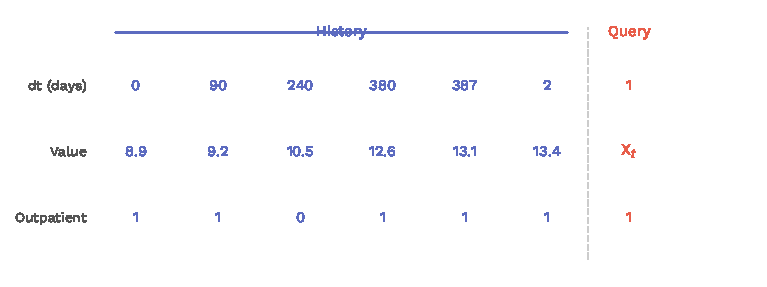
\includegraphics[width=\textwidth,height=0.78\textheight,keepaspectratio]{figures/token_example.pdf}
\caption{Example token sequence input to NORMA. Each measurement is represented by a time gap (days since previous), the lab value, and a binary outpatient indicator. The model predicts the distribution of the next value X\textsubscript{t}.}
\end{figure}
\clearpage

\begin{figure}[H]
\centering
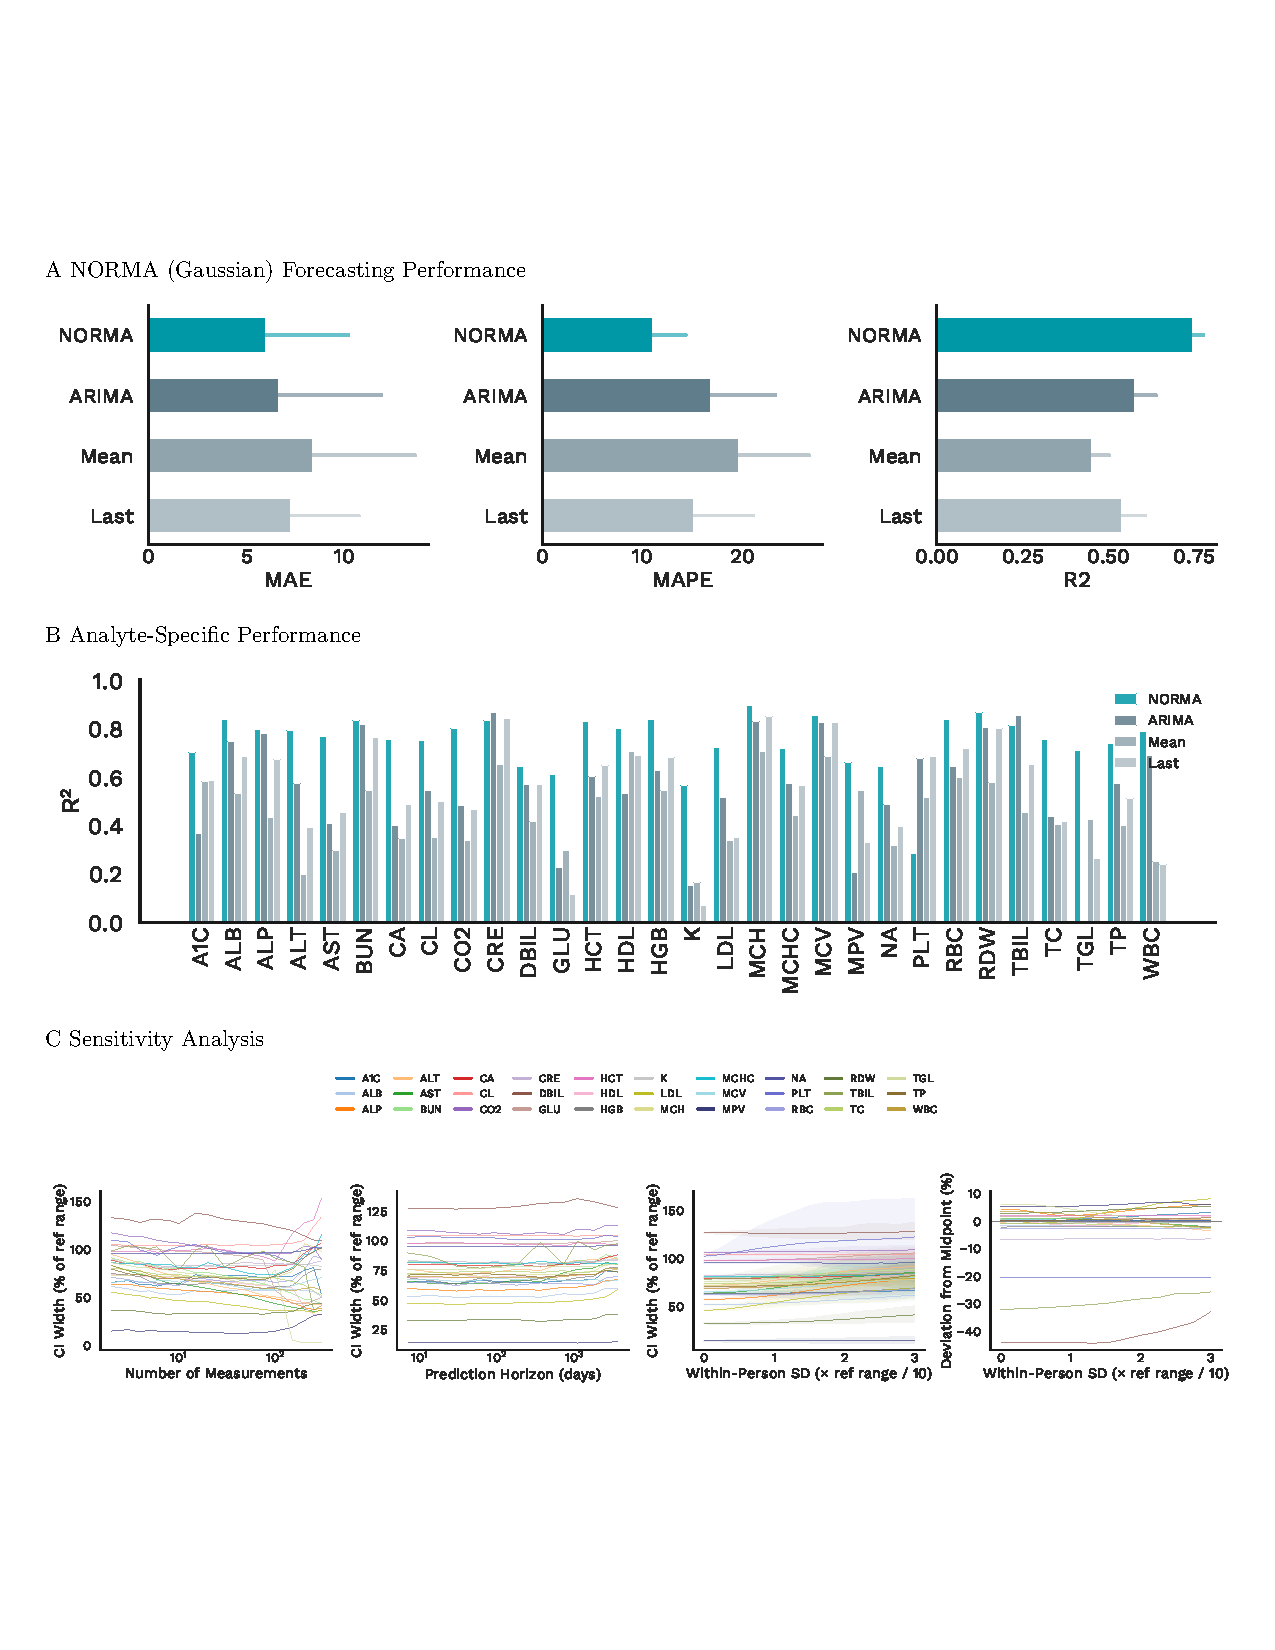
\includegraphics[width=\textwidth,height=0.78\textheight,keepaspectratio]{figures/supp_gaussian.pdf}
\caption{NORMA (Gaussian) predictive performance.
\textbf{(A)}~Forecasting accuracy (MAE, MAPE, R\textsuperscript{2}) compared with baselines.
\textbf{(B)}~Per-analyte R\textsuperscript{2}.
\textbf{(C)}~Sensitivity analysis: effect of history length, prediction horizon, and within-person variability.}
\end{figure}
\clearpage

\begin{figure}[H]
\centering
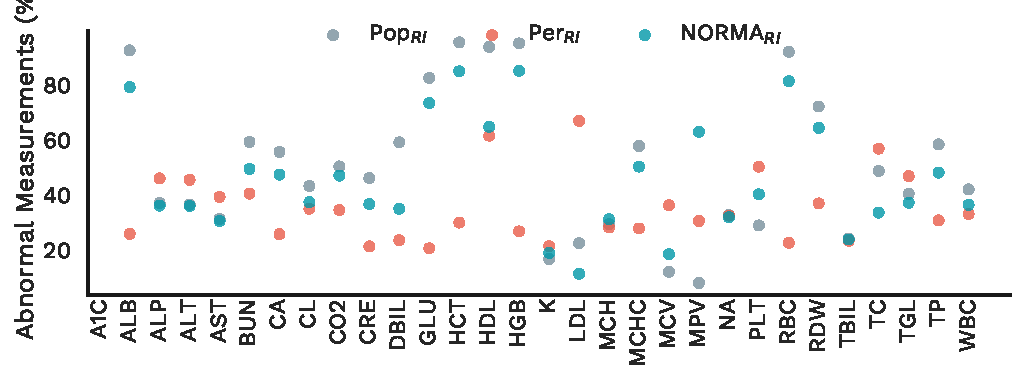
\includegraphics[width=\textwidth,height=0.38\textheight,keepaspectratio]{figures/eicu_prevalence.pdf}
\vspace{0.3cm}
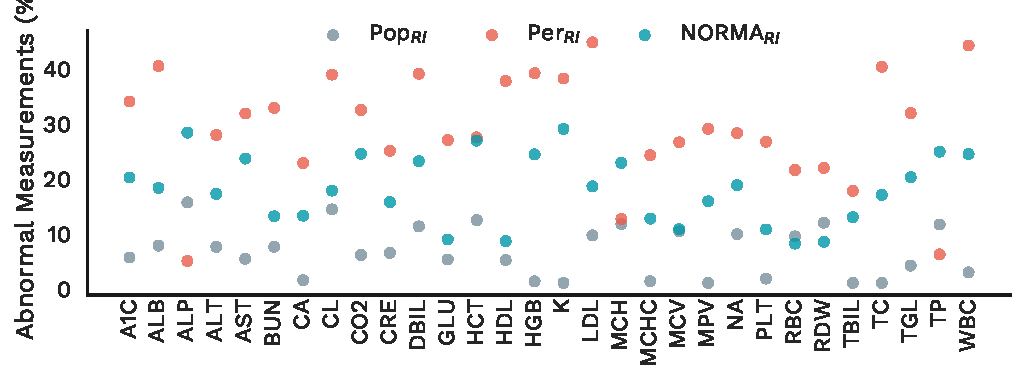
\includegraphics[width=\textwidth,height=0.38\textheight,keepaspectratio]{figures/chs_prevalence.pdf}
\caption{Abnormality prevalence across reference interval frameworks. Top: eICU. Bottom: CHS.}
\end{figure}
\clearpage

\begin{figure}[H]
\centering
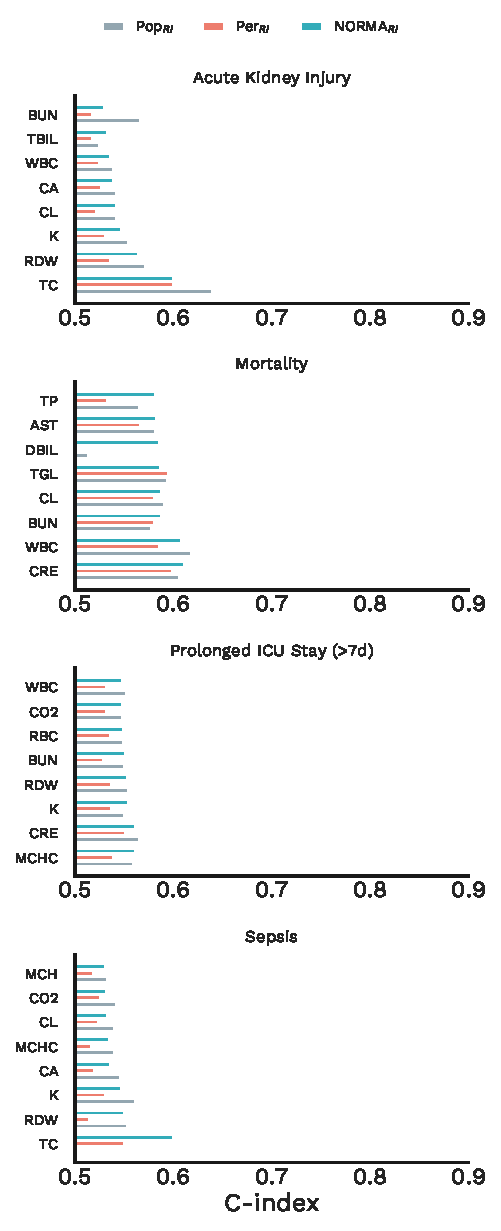
\includegraphics[width=\textwidth,height=0.78\textheight,keepaspectratio]{figures/cox_concordance.pdf}
\caption{Concordance index for Cox time-to-event models by analyte and method in eICU.}
\end{figure}
\clearpage

\begin{figure}[H]
\centering
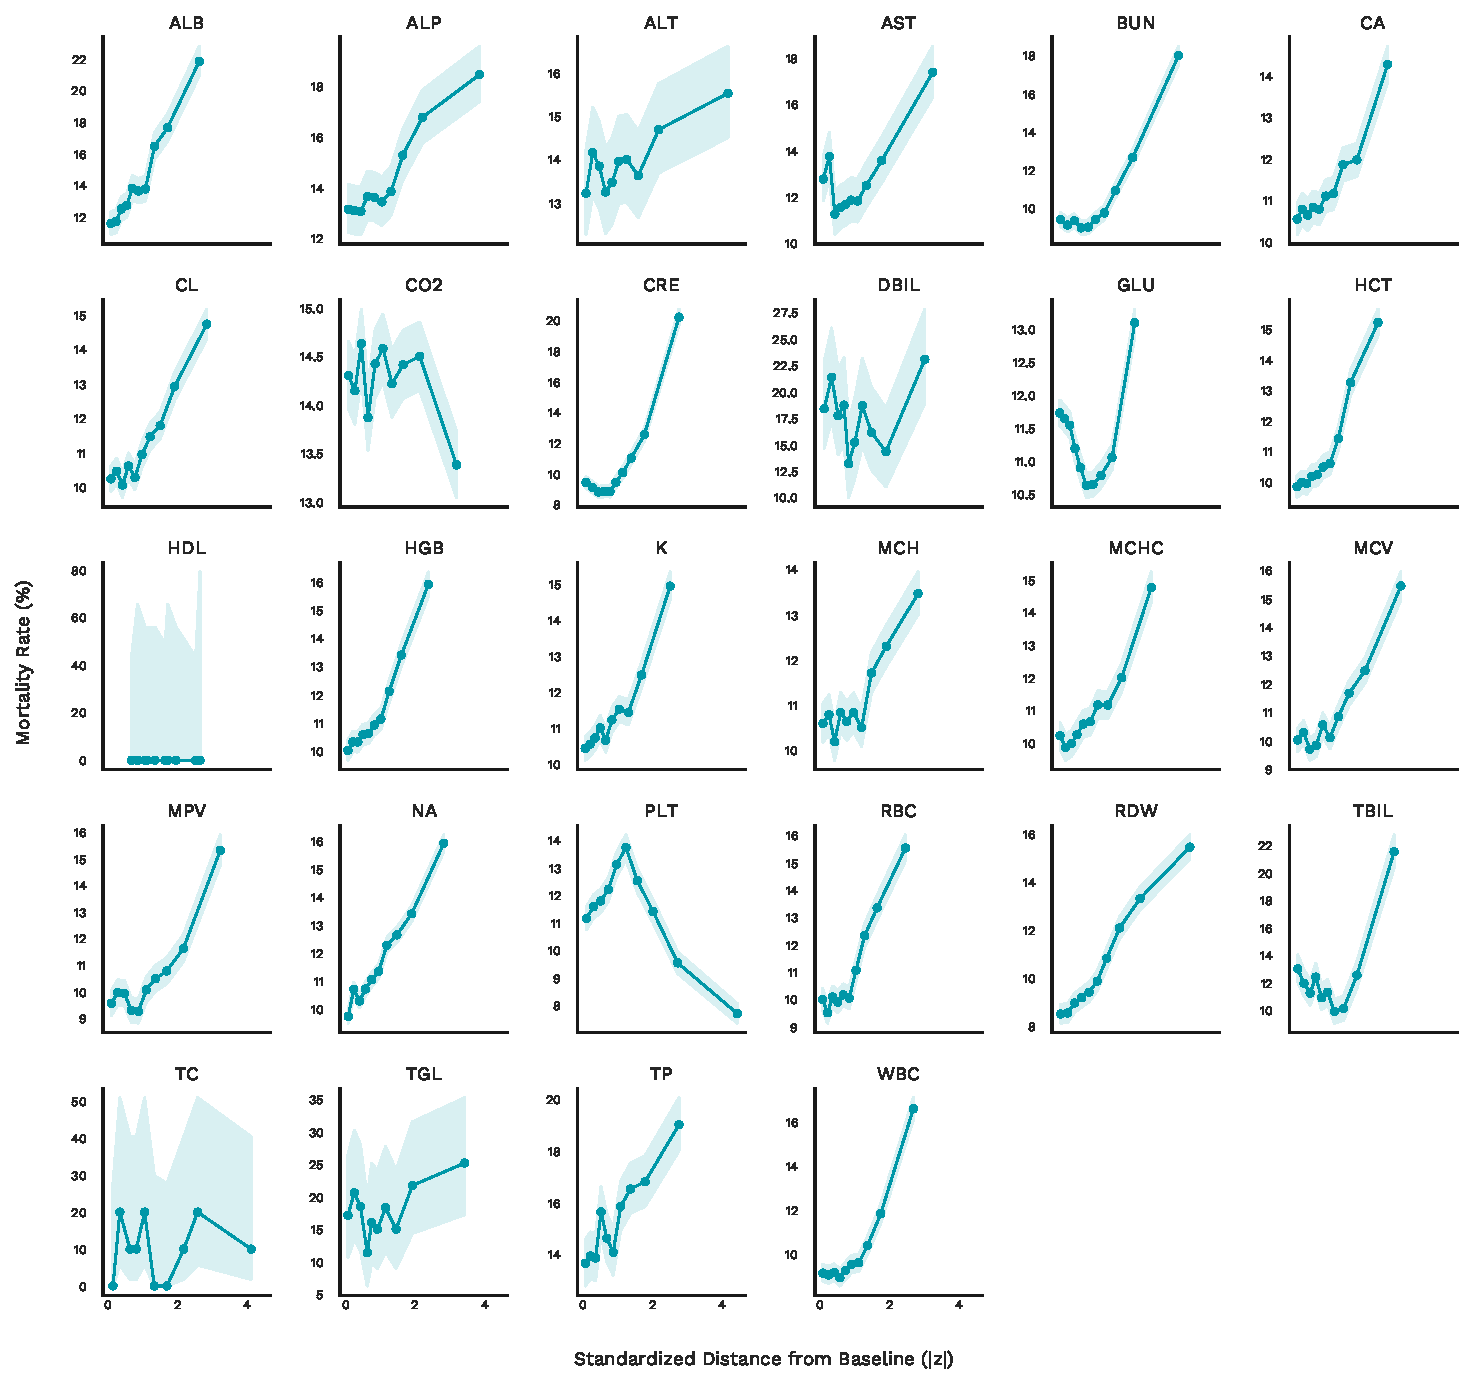
\includegraphics[width=\textwidth,height=0.78\textheight,keepaspectratio]{figures/mortality_by_deviation.pdf}
\caption{Mortality rate by standardized deviation from personal baseline in eICU.}
\end{figure}
\clearpage

\begin{figure}[H]
\centering
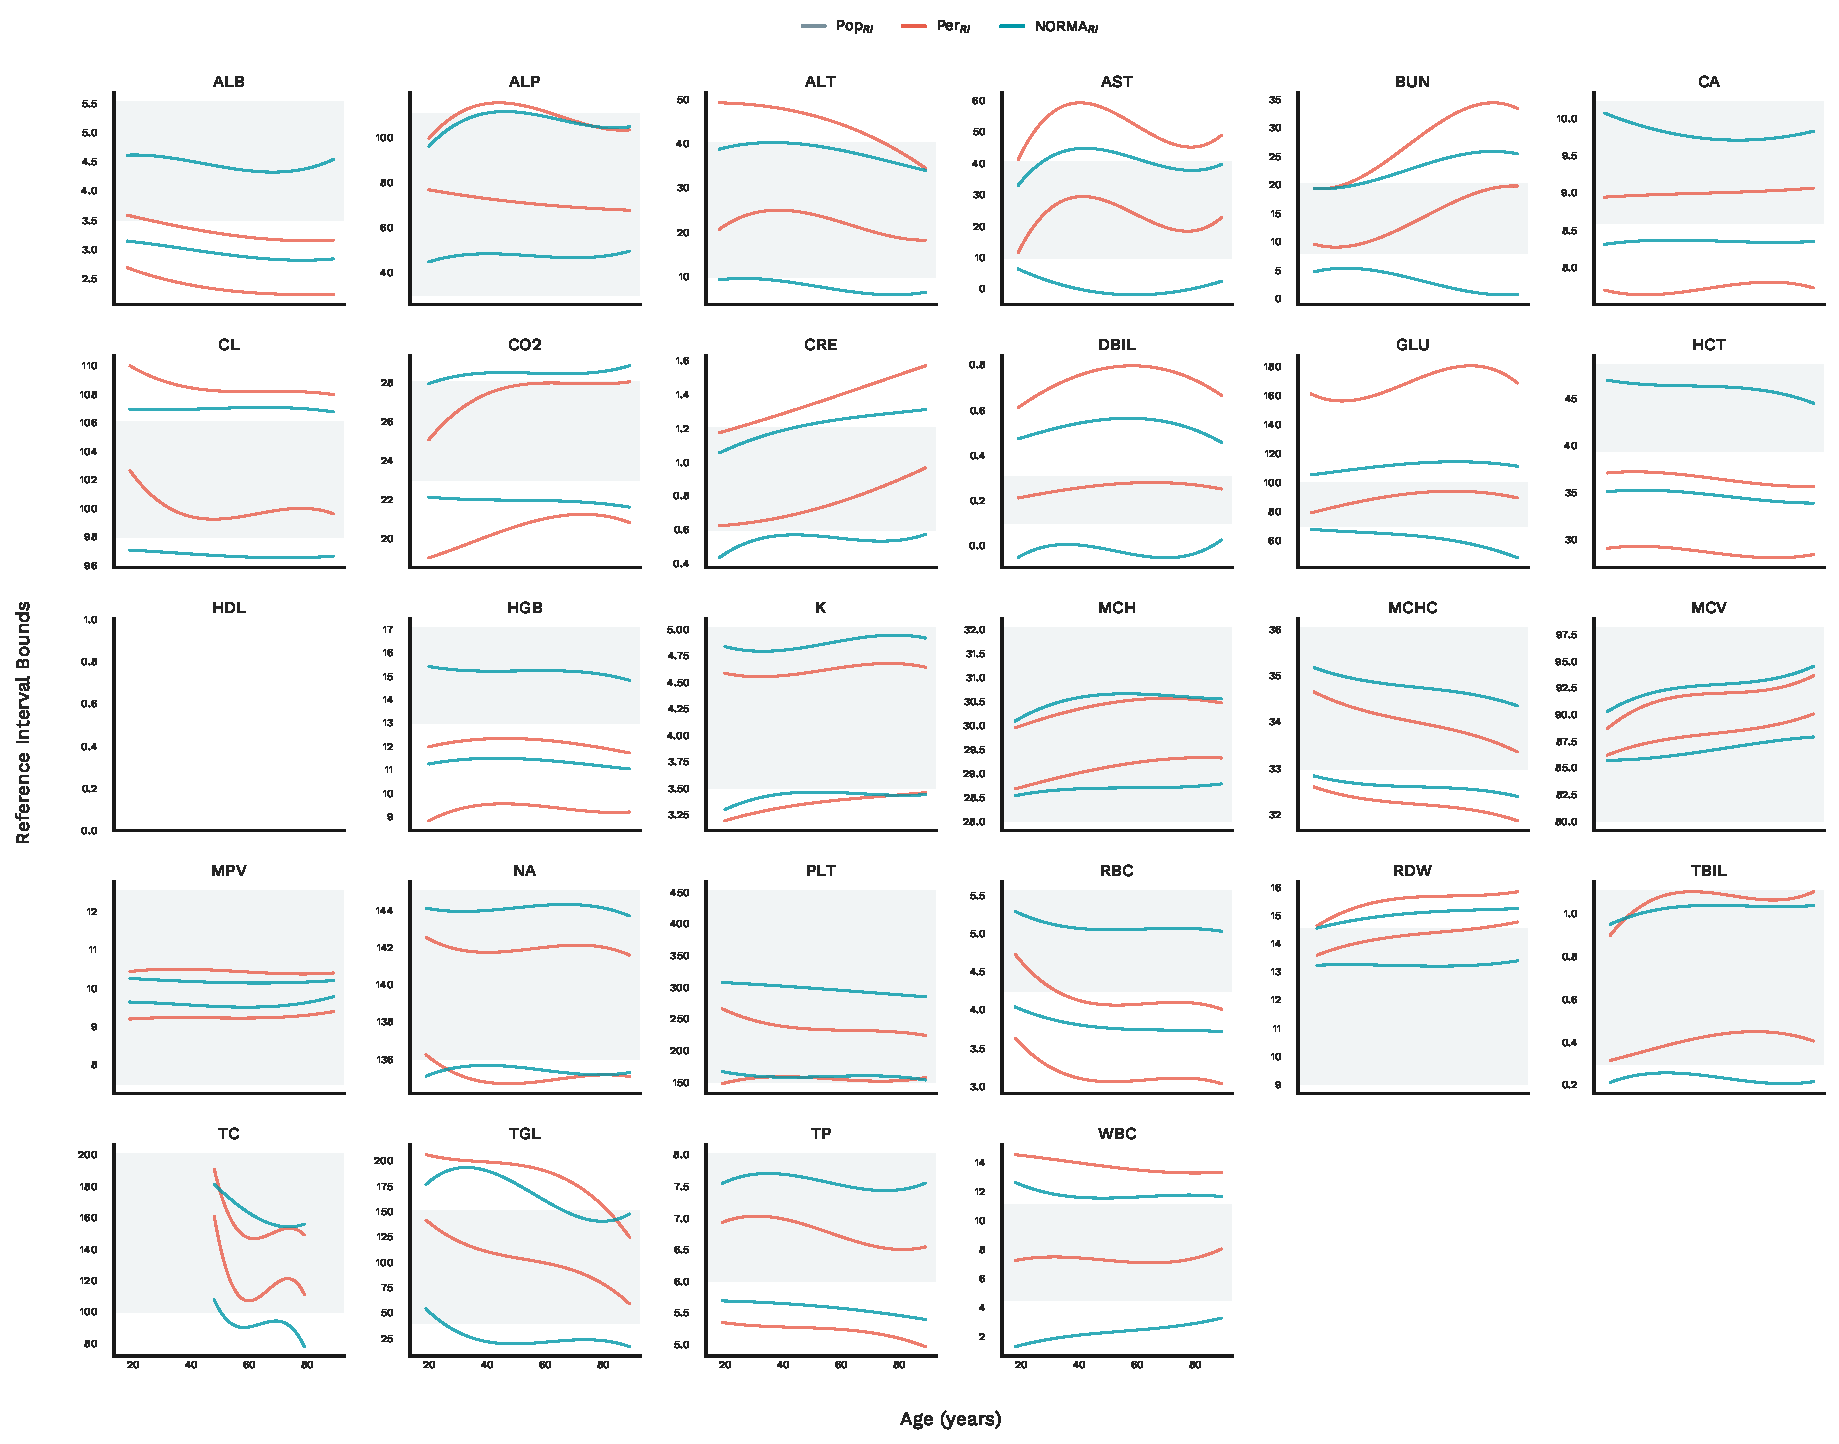
\includegraphics[width=\textwidth,height=0.78\textheight,keepaspectratio]{figures/age_ri.pdf}
\caption{Age-dependent reference interval trends in eICU.}
\end{figure}
\clearpage
